\subsection{Jet $\phi{}$ Resolution}
\label{GBJ2:JPhiR}

The effect of the jet $\phi$ resolution is assessed by smearing every jet's $\phi$ in the event by a Gaussian function, with the width found by comparing the $\phi$ of truth and reconstructed jets, which is calculated by another member of the analysis team. 
This method is an overestimate of the $\phi$ resolution uncertainty (ie $100\%$ uncertainty), but a data-driven method is not available in the forward region.
The effect is assessed in the same way as in Section \ref{GBJ2:JER}, using multiple smears and taking the average to reduce fluctuations. 
As no cuts are dependent on $\phi$, only distributions that are $\phi$ dependent are affected.

Figures \ref{GBJ2:ResoPhi:cos} -- \ref{GBJ2:ResoPhi:dphi78} show the ratio of the final distributions from the jets smeared by the Gaussian function and from the nominal jets.
The different blue histograms represent the 10 implementations of the increased jet $\phi$ resolution, the two red histogram are the uncertainty band found from the average of the blue histograms, and the black points show the PYTHIA statistical uncertainties.

Figure \ref{GBJ2:ResoPhi:cos} shows the ratio for \mean{\cosdphi{}} as a function of the dijet rapidity separation, \dy{}, for both (a) inclusive events and (b) gap events.
For both the gap and inclusive distributions, the increased $\phi$ smearing has reduced the \mean{\cosdphi{}} by about $1\%$ at low \dy{}, but at larger \dy{} the effect becomes small.
Figure \ref{GBJ2:ResoPhi:cos2} shows the ratio for \mean{\costwodphi{}} as a function of the dijet rapidity separation, \dy{}, for both (a) inclusive events and (b) gap events.
Again the effect is largest at low \dy{}, and the maximum uncertainty is  $2\%$. 

Figure \ref{GBJ2:ResoPhi:dphi23} shows the ratio for \dphiDist{} for (a) inclusive events and (b) gap events with $2<\dy{}<3$.
The effect of the $\phi$ smearing is around  $3\%$ for inclusive events and  $5\%$ for gap events.
Figure \ref{GBJ2:ResoPhi:dphi45} shows the ratio for \dphiDist{} for (a) inclusive events and (b) gap events with $4<\dy{}<5$.
The effect of the $\phi$ smearing is around  $2\%$ for inclusive events and  $3\%$ for gap events.
Figure \ref{GBJ2:ResoPhi:dphi78} shows the ratio for \dphiDist{} for (a) inclusive events and (b) gap events with $7<\dy{}<8$.
The effect of the $\phi$ smearing is around  $2\%$ for both the inclusive and gap events.
In the \dphi{} individual smeared ratios for all the \dy{} slices, the highest \dphi{} bin has lost events which have migrated into the other \dphi{} bins. 
This is expected due to the boundary of \dphi{} at one, and the steeply falling \dphi{} distribution.


\begin{figure}
\centering
        \begin{subfigure}[b]{0.5\textwidth}
                \centering
                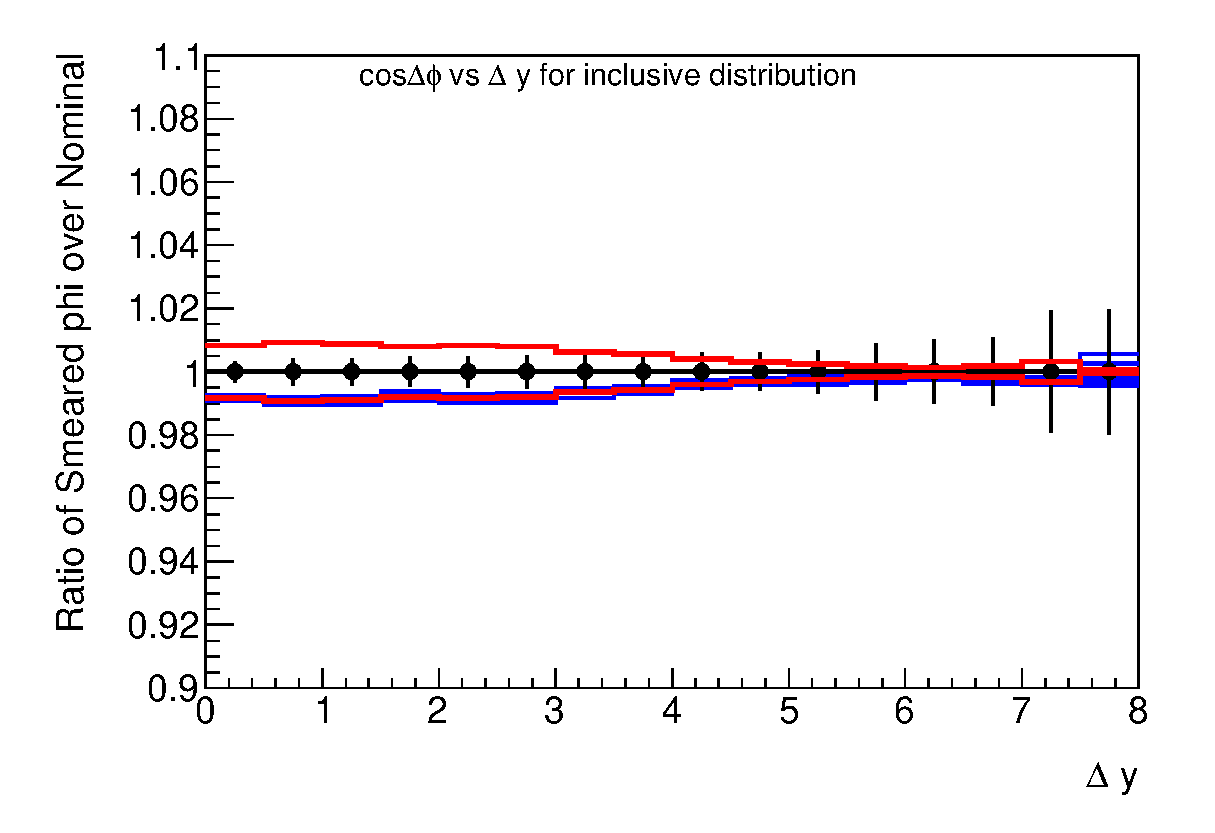
\includegraphics[width=\textwidth]{figures/GBJ2/ResoPhi/RMS_phi___cosdPhi_deltaY_Ratio.eps}
        \end{subfigure}%
        \begin{subfigure}[b]{0.5\textwidth}
                \centering
                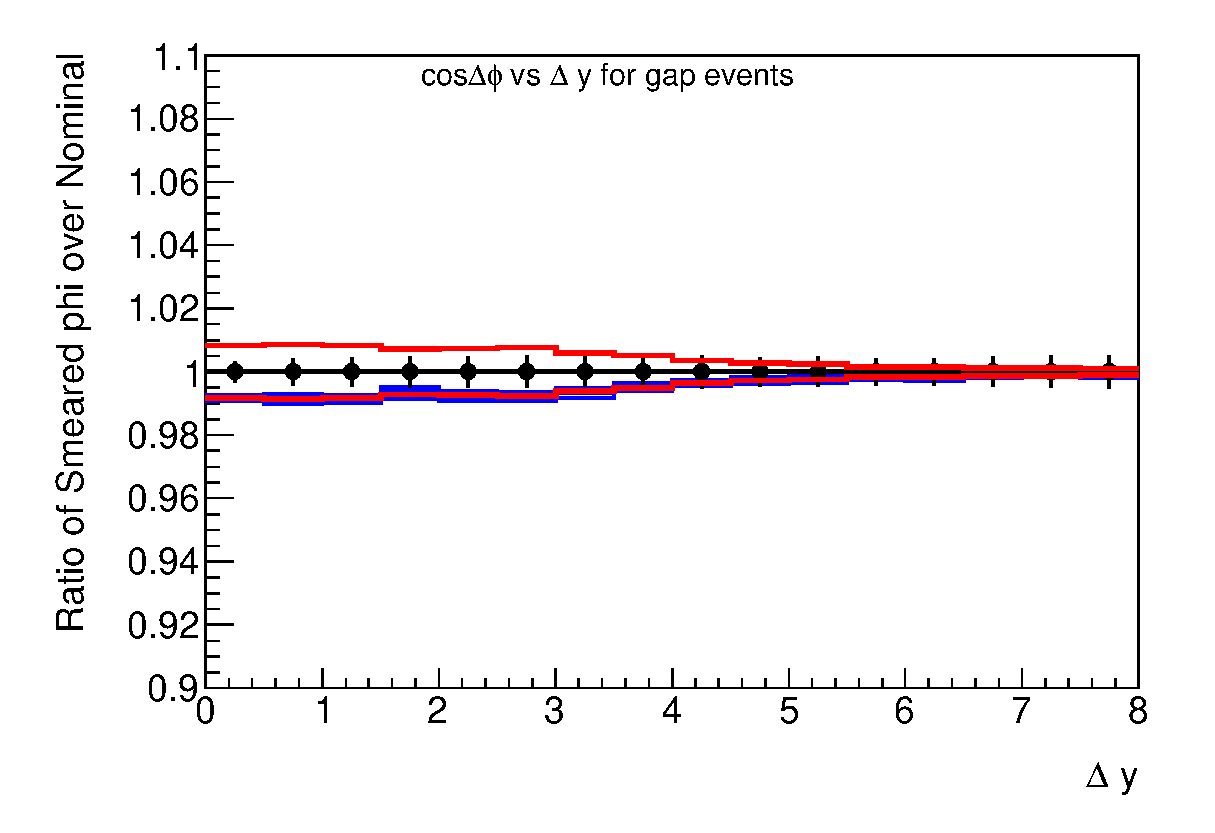
\includegraphics[width=\textwidth]{figures/GBJ2/ResoPhi/RMS_phi___cosdPhi_deltaY_gap_Ratio.eps}
        \end{subfigure}%

\caption[Uncertainty bands due to the jet $\phi$ resolution for \mean{\cosdphi{}}]{
The ratio of \mean{\cosdphi{}} as a function of \dy{} for (a) inclusive and (b) gap events reconstructed PYTHIA sample with nominal sample compared to $\phi$ smeared sample.
\label{GBJ2:ResoPhi:cos}}
\end{figure}

\begin{figure}
\centering
        \begin{subfigure}[b]{0.5\textwidth}
                \centering
                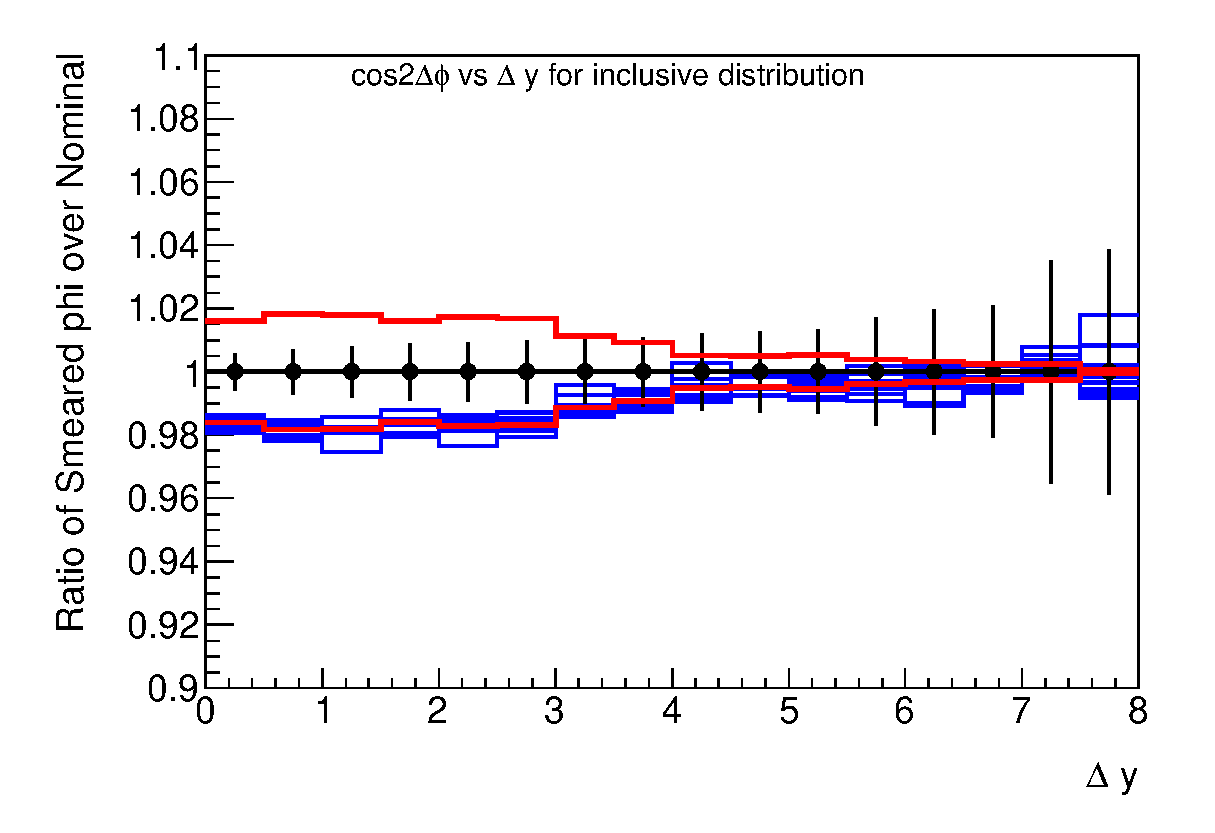
\includegraphics[width=\textwidth]{figures/GBJ2/ResoPhi/RMS_phi___cos2dPhi_deltaY_Ratio.eps}
        \end{subfigure}%
        \begin{subfigure}[b]{0.5\textwidth}
                \centering
                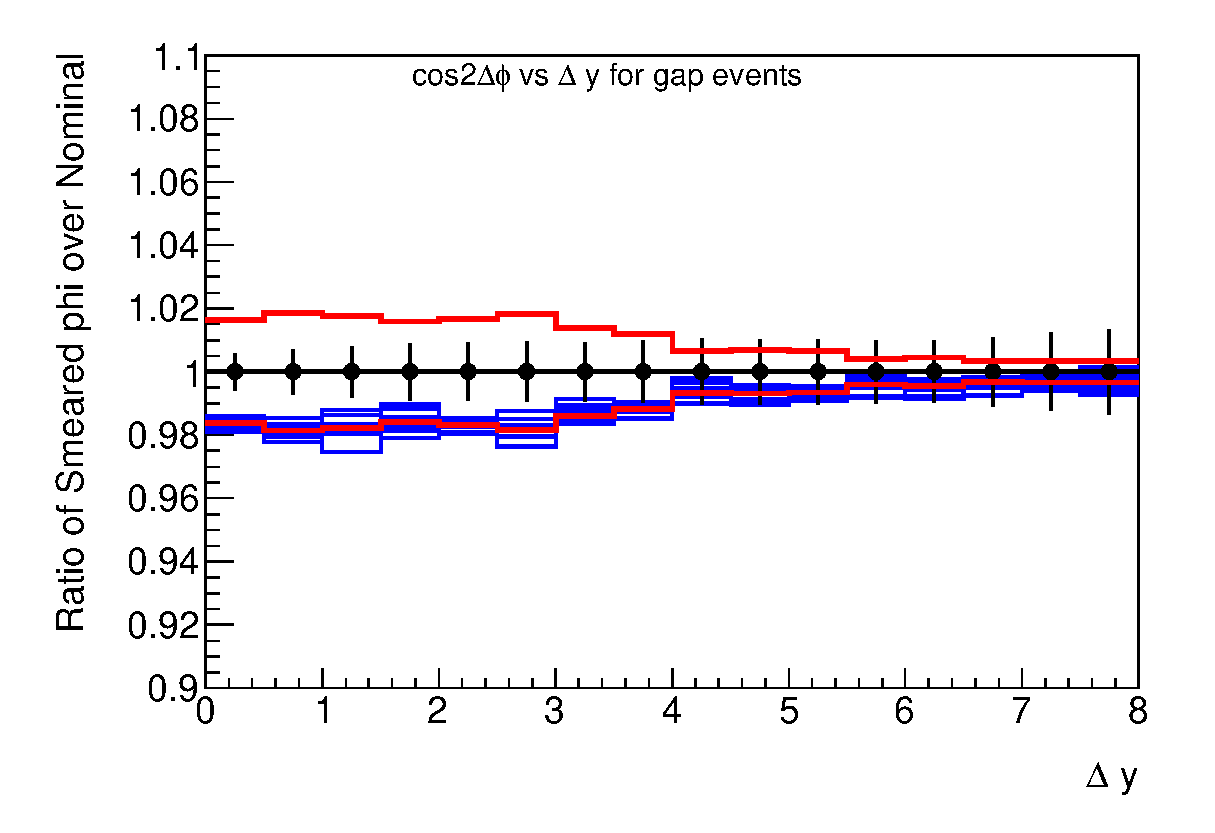
\includegraphics[width=\textwidth]{figures/GBJ2/ResoPhi/RMS_phi___cos2dPhi_deltaY_gap_Ratio.eps}
        \end{subfigure}%
\caption[Uncertainty bands due to the jet $\phi$ resolution for \mean{\costwodphi{}}]{
The ratio of \mean{\costwodphi{}} as a function of \dy{} for (a) inclusive and (b) gap events reconstructed PYTHIA sample with nominal sample compared to $\phi$ smeared sample.
\label{GBJ2:ResoPhi:cos2}}
\end{figure}


\begin{figure}
\centering
        \begin{subfigure}[b]{0.5\textwidth}
                \centering
                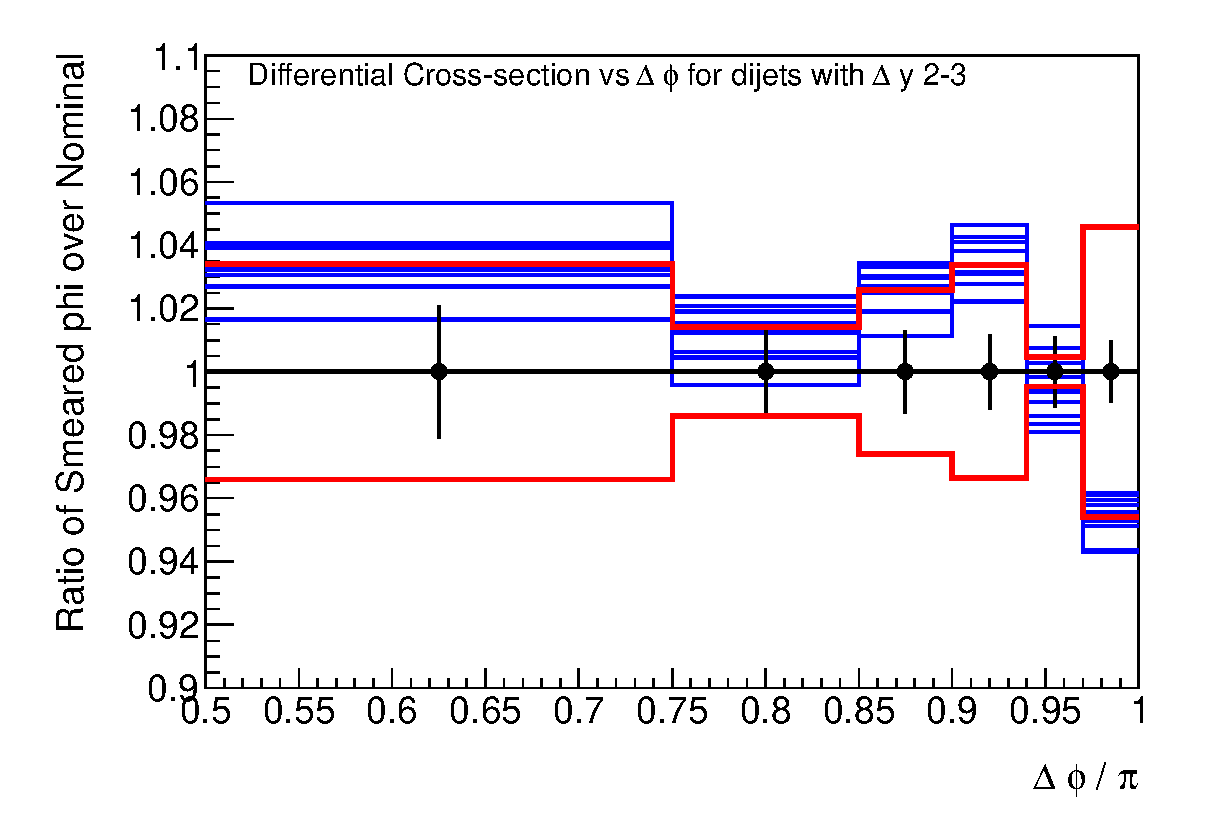
\includegraphics[width=\textwidth]{figures/GBJ2/ResoPhi/RMS_phi___dPhi__2_3_Ratio.eps}
        \end{subfigure}%
        \begin{subfigure}[b]{0.5\textwidth}
                \centering
                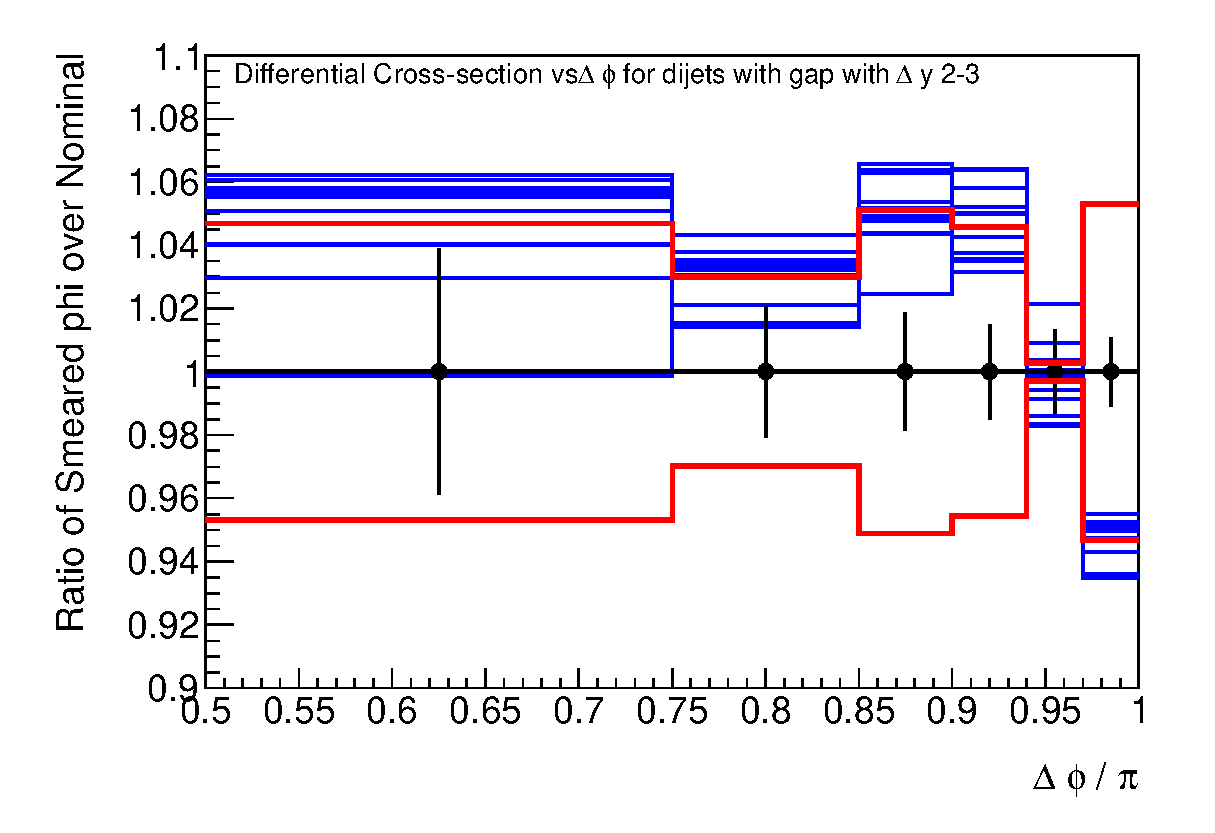
\includegraphics[width=\textwidth]{figures/GBJ2/ResoPhi/RMS_phi___dPhi_gap__2_3_Ratio.eps}
        \end{subfigure}%
\caption[Uncertainty bands due to the jet $\phi$ resolution for \dphiDist{} for $2<\dy{}<3$]{
The ratio of \dphiDist{} for $2<\dy{}<3$ for (a) inclusive and (b) gap events reconstructed PYTHIA sample with nominal sample compared to $\phi$ smeared sample.
\label{GBJ2:ResoPhi:dphi23}}
\end{figure}


\begin{figure}
\centering
        \begin{subfigure}[b]{0.5\textwidth}
                \centering
                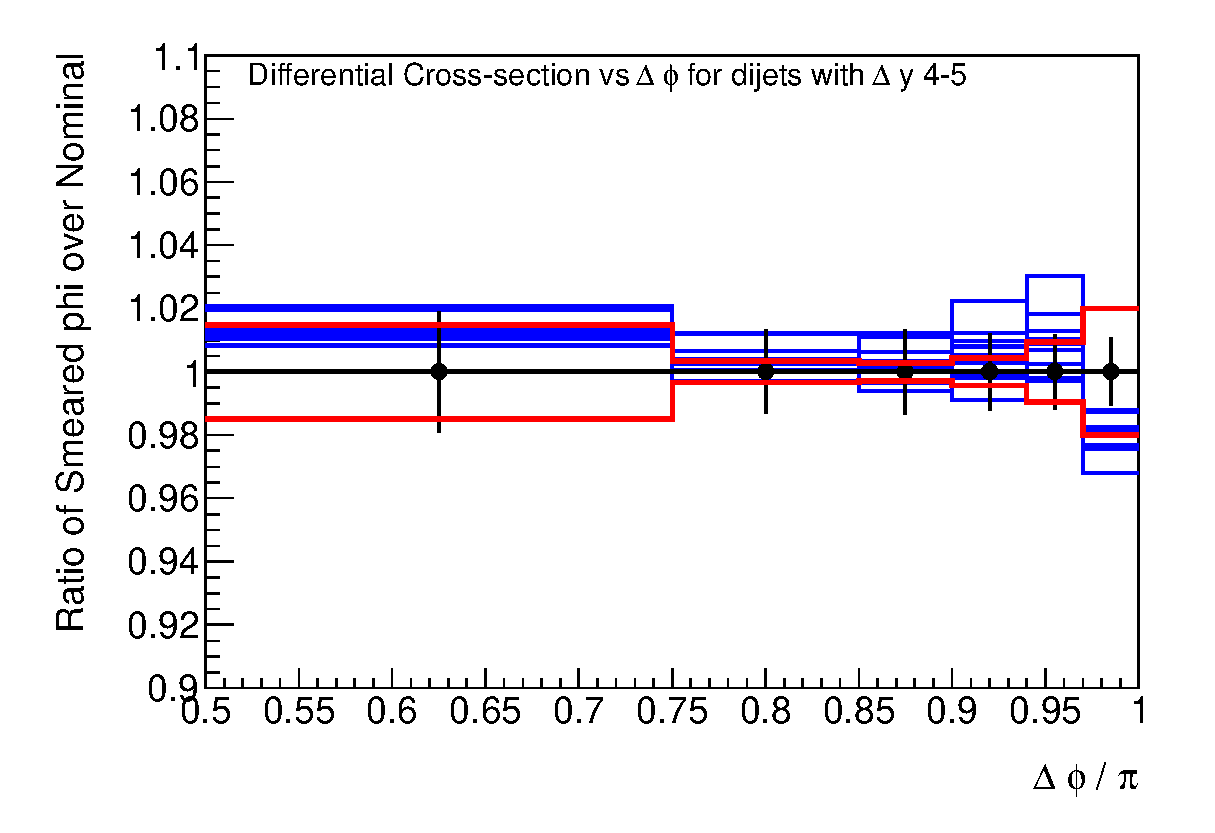
\includegraphics[width=\textwidth]{figures/GBJ2/ResoPhi/RMS_phi___dPhi__4_5_Ratio.eps}
        \end{subfigure}%
        \begin{subfigure}[b]{0.5\textwidth}
                \centering
                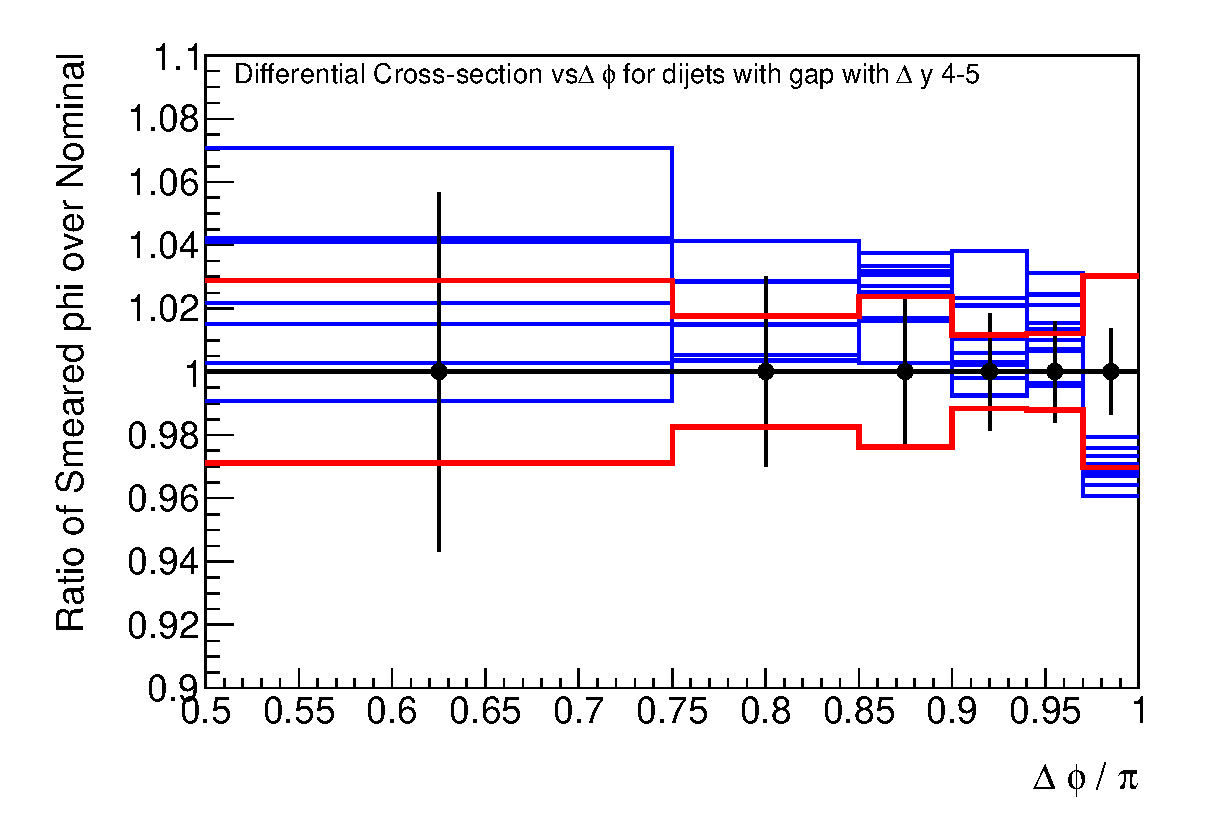
\includegraphics[width=\textwidth]{figures/GBJ2/ResoPhi/RMS_phi___dPhi_gap__4_5_Ratio.eps}
        \end{subfigure}%
\caption[Uncertainty bands due to the jet $\phi$ resolution for \dphiDist{} for $4<\dy{}<5$]{
The ratio of \dphiDist{} for $4<\dy{}<5$ for (a) inclusive and (b) gap events reconstructed PYTHIA sample with nominal sample compared to $\phi$ smeared sample.
\label{GBJ2:ResoPhi:dphi45}}
\end{figure}



\begin{figure}
\centering
        \begin{subfigure}[b]{0.5\textwidth}
                \centering
                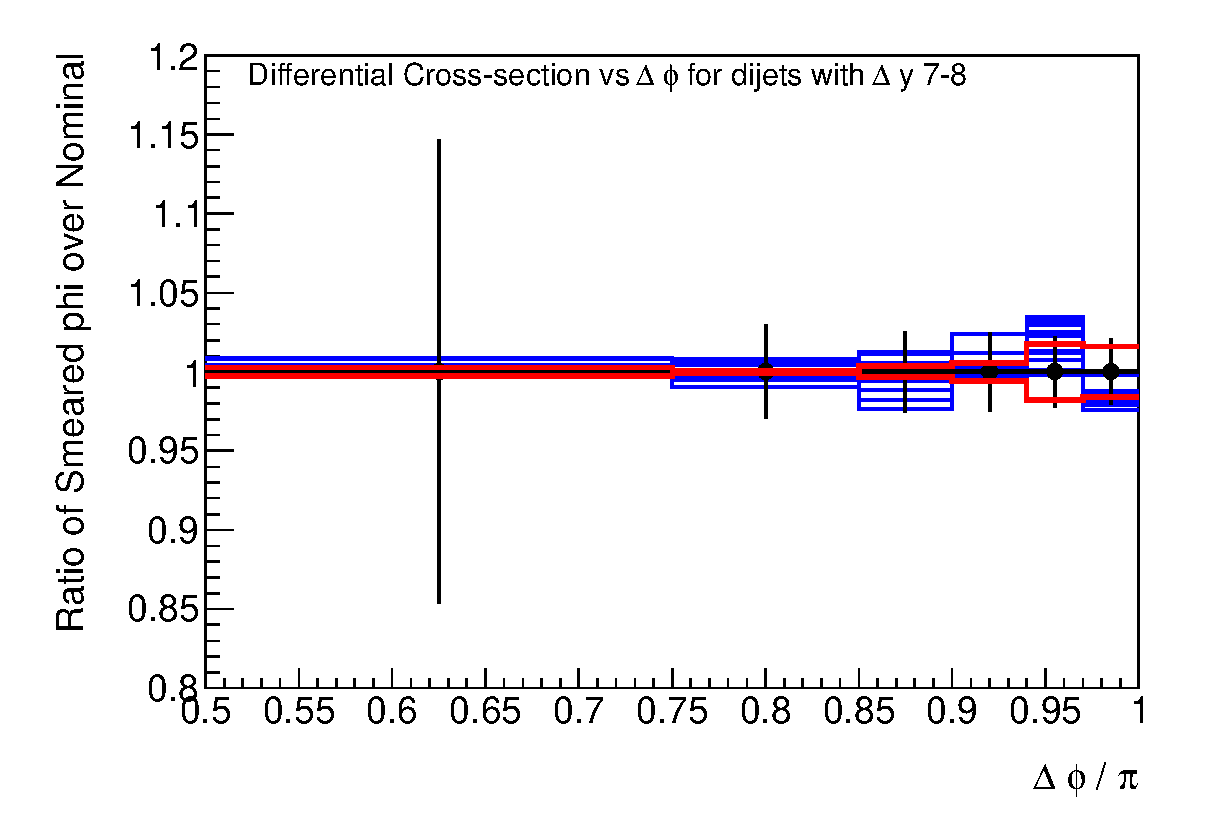
\includegraphics[width=\textwidth]{figures/GBJ2/ResoPhi/RMS_phi___dPhi__7_8_Ratio.eps}
        \end{subfigure}%
        \begin{subfigure}[b]{0.5\textwidth}
                \centering
                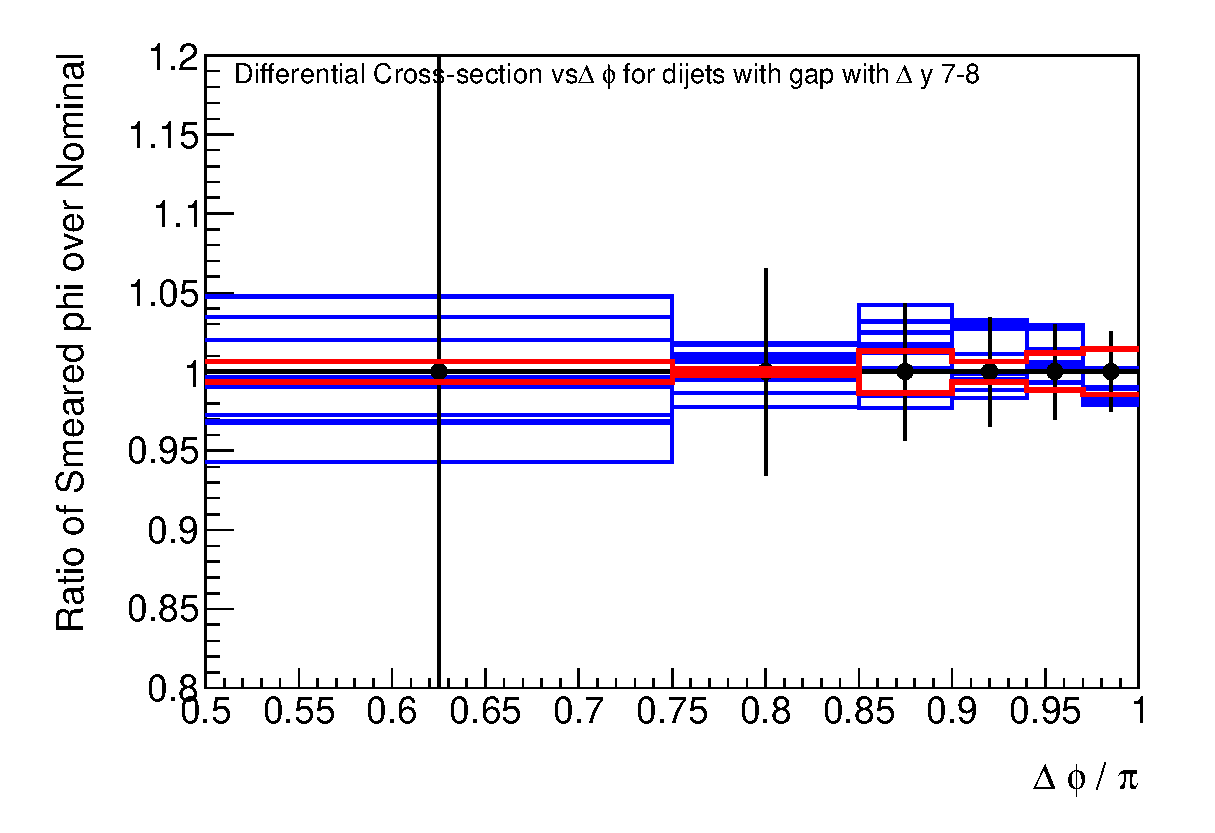
\includegraphics[width=\textwidth]{figures/GBJ2/ResoPhi/RMS_phi___dPhi_gap__7_8_Ratio.eps}
        \end{subfigure}%
\caption[Uncertainty bands due to the jet $\phi$ resolution for \dphiDist{} for $7<\dy{}<8$]{
The ratio of \dphiDist{} for $7<\dy{}<8$ for (a) inclusive and (b) gap events reconstructed PYTHIA sample with nominal sample compared to $\phi$ smeared sample.
\label{GBJ2:ResoPhi:dphi78}}
\end{figure}


